% This is "sig-alternate.tex" V1.8 June 2007 Modified for SOUPS 2014
% This file should be compiled with V2.3 of "sig-alternate.cls" June 2007
%
% This example file demonstrates the use of the 'sig-alternate.cls'
% V2.3 LaTeX2e document class file. It is for those submitting
% articles to ACM Conference Proceedings WHO DO NOT WISH TO
% STRICTLY ADHERE TO THE SIGS (PUBS-BOARD-ENDORSED) STYLE.
% The 'sig-alternate.cls' file will produce a similar-looking,
% albeit, 'tighter' paper resulting in, invariably, fewer pages.
%
% ----------------------------------------------------------------------------------------------------------------
% This .tex file (and associated .cls V2.3) produces:
%       1) The Permission Statement
%       2) The Conference (location) Info information
%       3) The Copyright Line with ACM data
%       4) NO page numbers
%
% as against the acm_proc_article-sp.cls file which
% DOES NOT produce 1) thru' 3) above.
%
% Using 'sig-alternate.cls' you have control, however, from within
% the source .tex file, over both the CopyrightYear
% (defaulted to 200X) and the ACM Copyright Data
% (defaulted to X-XXXXX-XX-X/XX/XX).
% e.g.
% \CopyrightYear{2007} will cause 2007 to appear in the copyright line.
% \crdata{0-12345-67-8/90/12} will cause 0-12345-67-8/90/12 to appear in the copyright line.
%
% ---------------------------------------------------------------------------------------------------------------
% This .tex source is an example which *does* use
% the .bib file (from which the .bbl file % is produced).
% REMEMBER HOWEVER: After having produced the .bbl file,
% and prior to final submission, you *NEED* to 'insert'
% your .bbl file into your source .tex file so as to provide
% ONE 'self-contained' source file.
%
% ================= IF YOU HAVE QUESTIONS =======================
% Questions regarding the SIGS styles, SIGS policies and
% procedures, Conferences etc. should be sent to
% Adrienne Griscti (griscti@acm.org)
%
% Technical questions _only_ to
% Gerald Murray (murray@acm.org)
% ===============================================================
%
% For tracking purposes - this is V1.8 - June 2007

% --- Start page size ---
%Please use the following format  
\documentclass{soups} 
\pdfpagewidth=8.5truein 
\pdfpageheight=11truein 
% --- End page size ---


\usepackage{graphicx}
\usepackage{times}
\usepackage{url}
\usepackage{color}
\usepackage{booktabs}
\usepackage{float}

\renewcommand{\topfraction}{0.99} % be more aggressive about text around floats
\renewcommand{\floatpagefraction}{0.99}
\pagestyle{plain} % page numbers



\begin{document}
%
% --- Author Metadata here ---
\conferenceinfo{Conference}{year, month dates, city, state.}
\CopyrightYear{2017} % Allows default copyright year (200X) to be over-ridden - IF NEED BE.
%\crdata{0-12345-67-8/90/01}  % Allows default copyright data (0-89791-88-6/97/05) to be over-ridden - IF NEED BE.
% --- End of Author Metadata ---

\title{Detecting Phone Theft Using Machine Learning}
% \titlenote{(Produces the permission block, and copyright information). For use with SIG-ALTERNATE.CLS. Supported by ACM.}}
% \subtitle{Subtitle (optional)%
% \titlenote{A full version of this paper is available as
% \textit{Author's Guide to Preparing ACM SIG Proceedings Using
% \LaTeX$2_\epsilon$\ and BibTeX} at
% \texttt{www.acm.org/sigs/publications/sigguide-v2.2sp}}}
%
% You need the command \numberofauthors to handle the 'placement
% and alignment' of the authors beneath the title.
%
% For aesthetic reasons, we recommend 'three authors at a time'
% i.e. three 'name/affiliation blocks' be placed beneath the title.
%
% NOTE: You are NOT restricted in how many 'rows' of
% "name/affiliations" may appear. We just ask that you restrict
% the number of 'columns' to three.
%
% Because of the available 'opening page real-estate'
% we ask you to refrain from putting more than six authors
% (two rows with three columns) beneath the article title.
% More than six makes the first-page appear very cluttered indeed.
%
% Use the \alignauthor commands to handle the names
% and affiliations for an 'aesthetic maximum' of six authors.
% Add names, affiliations, addresses for
% the seventh etc. author(s) as the argument for the
% \additionalauthors command.
% These 'additional authors' will be output/set for you
% without further effort on your part as the last section in
% the body of your article BEFORE References or any Appendices.

% \numberofauthors{3} %  in this sample file, there are a *total*
% of EIGHT authors. SIX appear on the 'first-page' (for formatting
% reasons) and the remaining two appear in the \additionalauthors section.
%
% \author{
% You can go ahead and credit any number of authors here,
% e.g. one 'row of three' or two rows (consisting of one row of three
% and a second row of one, two or three).
%
% The command \alignauthor (no curly braces needed) should
% precede each author name, affiliation/snail-mail address and
% e-mail address. Additionally, tag each line of
% affiliation/address with \affaddr, and tag the
% e-mail address with \email.
%
% 1st. author
% \alignauthor
% Xinyu Liu \\
%        \affaddr{UC Berkeley} \\
%        \email{xinyuliu@berkeley.edu}
% % 2nd. author
% \alignauthor
% David Wagner \\
%        \affaddr{UC Berkeley} \\
%        \email{daw@cs.berkeley.edu}
% % 3rd. author
% \alignauthor 
% Serge Egelman \\
%        \affaddr{UC Berkeley, ICSI} \\
%        \email{egelman@cs.berkeley.edu}
% \and  % use '\and' if you need 'another row' of author names
% % 4th. author
% \alignauthor Lawrence P. Leipuner\\
%        \affaddr{Brookhaven Laboratories}\\
%        \affaddr{Brookhaven National Lab}\\
%        \affaddr{P.O. Box 5000}\\
%        \email{lleipuner@researchlabs.org}
% % 5th. author
% \alignauthor Sean Fogarty\\
%        \affaddr{NASA Ames Research Center}\\
%        \affaddr{Moffett Field}\\
%        \affaddr{California 94035}\\
%        \email{fogartys@amesres.org}
% % 6th. author
% \alignauthor Charles Palmer\\
%        \affaddr{Palmer Research Laboratories}\\
%        \affaddr{8600 Datapoint Drive}\\
%        \affaddr{San Antonio, Texas 78229}\\
%        \email{cpalmer@prl.com}
% }
% There's nothing stopping you putting the seventh, eighth, etc.
% author on the opening page (as the 'third row') but we ask,
% for aesthetic reasons that you place these 'additional authors'
% in the \additional authors block, viz.
% \additionalauthors{Additional authors: John Smith (The Th{\o}rv{\"a}ld Group,
% email: {\texttt{jsmith@affiliation.org}}) and Julius P.~Kumquat
% (The Kumquat Consortium, email: {\texttt{jpkumquat@consortium.net}}).}
% \date{30 July 1999}
% Just remember to make sure that the TOTAL number of authors
% is the number that will appear on the first page PLUS the
% number that will appear in the \additionalauthors section.

\maketitle
\begin{abstract}
Millions of smartphones are stolen in the United States every year, putting victims' personal information at risk since many users often do not lock their phones. 
To protect individuals' smartphones and the private data stored on them, we develop a system that automatically detects pickpocket and grab-and-run theft, where a thief grabs the phone from a victim's hand then runs away. 
Our system applies machine learning to smartphone accelerometer data. Based on a field study and simulated theft scenarios, we are able to detect all thefts at a cost of 1 false alarm per week.
\end{abstract}




\section{Introduction}
According to Consumer Reports, 2.1 million smartphones were stolen in the United States in 2014 \cite{deitrick:consumer}, and the Pew Research Center's Internet \& American Life Project reported in 2012 that nearly one third of mobile phone users have experienced a lost or stolen devices \cite{boyles:pew}.
People can lock their phones to mitigate the risks of phone theft, but this is less convenient as it requires unlocking their phone every time they want to use their phone.
Consequently, about 40\% of smartphone users do not lock their phones, which allows thieves to gain access to the victims' personal information \cite{egelman:lock}.

In this paper, we develop a method to automatically detect detect pickpocket and grab-and-run smartphone theft. To be more specific, we train a binary classifier to recognize the movements that are specific to theft and use it monitor accelerometer data in the background.
When theft is detected, it can signal the device to lock the phone and notify the owner. Thus, our theft detector offers another layer of protection against smartphone theft.
Because our detector is completely automatic, it is convenient for users.

There are multiple ways that a phone might be stolen.
We focus specifically on grab-and-run theft, where the thief snatches the phone out of the user's hand and runs away, and pickpocket theft, where the thief steals the phone from the user's pocket or bag and runs away.
This creates an abrupt and unusual movement pattern, which we show can be detected from analysis of accelerometer sensor data.
We do not attempt to detect other forms of theft, such as where the phone is left unattended and the thief walks off with it, or where the phone is lost or left behind somewhere.
Consequently, our scheme cannot offer comprehensive protection against all forms of theft, but we hope that it will be useful nonetheless.

We measure the effectiveness of our scheme by gathering two datasets.
First, we simulated three types of phone theft: grab-and-run while the victim is standing still, grab-and-run while the victim is walking at a constant speed, and pick-pocket theft.
We collect accelerometer sensor readings during the simulated thefts; these serve as known positives.
Second, we conducted a field study where we collected 3 weeks of sensor readings from the phones of 53 participants during their everyday life.
No phone was stolen during the field study, so these serve as known negatives.
We use this to train a classifier and then evaluate its detection rate and false positive rate.
Our best classifier produces 1 false alarm per week while detecting 100\% of simulated thefts.


Our contributions are:
\begin{enumerate}
  \item We conduct a user study and collect a large dataset of smartphone sensor data while devices are being used in real world.
  \item We devise features and methods to detect theft, and we show that it can detect thefts with few false positives.
\end{enumerate}




\section{Related Work}

The use of intrinsic sensor data to improve the security of smart devices and offer a way of continuous user authentication has drawn more and more attention recently. 
The embedded sensors on a smartphone have been used to develop biometric identification and authentication techniques. 
The major benefit of using smartphone-based biometric is to allow authentication to happen unobtrusively, i.e. not requiring any users action. 
We are particularly interested in research done to study gait recognition by mining the embedded accelerometer data on smartphones. 
For the purpose of our research, we emphasize on the feature extraction methods used in the previous work.

The unobtrusive biometric gait recognition technique introduced by Derawi et al. uses accelerometer data collected on smartphones from 51 subjects in the context of a laboratory setup for continuous authentication and results in a high equal error rate of 20\% \cite{derawi:gait}. 
They applied time interpolation and weighted moving average filter to clean the raw accelerometer data before extracting accelerometer measurements in average cycles as features.

Primo et al. further investigate and show that accelerometer-based gait authentication is somewhat dependent on the position in which the phone is held, which is a challenge for deploying gait authentication outside of a laboratory environment \cite{primo:context}. 
They preprocessed the raw measurements of X, Y, Z and magnitude (M) of the accelerometer data by a moving average of a 3 point window to mitigate sensor noise. 
They broke the resulting time series into windows, each containing 100 points and having an overlap of 50 points with the next window. 
They extracted and selected a set of top ranking features from X, Y, Z and M in each window to first determine phone position, then another set of highest ranked features to identify users. 
Their system was trained and achieved 80\% accuracy in user identification on data from 30 subjects.

Juefei-Xu et al. researched ways to identify human walking patterns at normal and fast pace using accelerometer on a smartphone \cite{xu:pace}. 
The acceleration is collected from 36 subjects walking at two different paces in a laboratory environment. 
They extracted feature vectors by concatenating x, y, z accelerations in two different intervals. 
One is a 3-second window centered around every spike in z acceleration. 
They also concatenated x, y, z accelerations from intervals between adjacent spikes after normalizing data in each interval to 500 samples. 
In addition, they applied signal processing methods to extracted and selected discriminative features. 
Their system achieved over 95\% accuracy when it was both trained and tested on two same-pace datasets. 
The system identified subjects walking at fast pace with 61\% accuracy when it was trained on data from the same subjects walking at normal pace.

Kwapisz et al collected a dataset of 36 subjects instructed by the researchers to perform 4 specific daily activities, walking, jogging, ascending and descending stairs \cite{kwapisz:biometrics}. 
They extracted features, mean, standard deviation, mean absolute difference, mean of magnitude, time between peaks, and binned distribution from 10-second intervals and use decision tree and neural network identify individual users. 
They achieve 90\% accuracy using 10 second worth of data from one of the activities, walking. 
They also built a binary classifier for each subject to match a query to a particular user for the purpose of user authentication and achieved over 80\% accuracy on positive authentication and over 90\% accuracy on negative authentication.

In addition to gait, Feng et al investigated using pickup motion as a biometic modality for user authentication \cite{feng:pickup}. 
They explored two methods to extract features from accelerometer, gyroscope and magnetometer data. 
In the statistical method, they used a move average filter to smooth raw data, then extracted temporal and numerical features, i.e. duration time, mean, variance, and standard derivation after normalization and segmentation. 
They used SVM to classify if given data is from a specific user. 
They also used data from multiple sessions to reconstruct pickup motion trajectories and a distance metric to distinguishes trajectories of different users. 
They tested their proposed method on a dataset of 31 subejcts performing pickup motion while standing and walking achieved equal error rate of 6.13\% and 7.09\% respectively.

The most relevant work is done by Chang et al in using pickup motion from pockets or single-shoulder bags as a biometric modality, uniquely associated to the owner, to detect smartphone theft in real-time \cite{cheng:theft}. 
Their authentication system prevents pickpocket smartphone thefts by analyzing accelerometer and gyroscope data to detect illegal pickup of a smartphone. 
Our acceleration-based approach detects pickpocket as well as grab-and-run thefts when the phone is in the possesion of the owner. 
They preprocessed raw accelerometer and gyroscope data by removing high freqency noise. 
They integrated six weak classifier trained by data from each of six dimenstions of accelerometer and gyroscope into one strong classifier then use the strong classifier to determine the legitimacy of picking up motions of a user. 
Their system achieved 10.2\% false positive rate and 5.5\% false negative rate on average. \textcolor{red}{ [need to covert these rates to comparable results to our work, but the author did not provide the number of negative samples used in test.]} 

The aforementioned acceleration-based approaches for gait recognistion have a common procedure. 
They first preprocess the noisy raw sensor data usig a filter, then segment and extract feature vectors from windows to be used for a classification algorithm. 
While an accelerometer-based biometric modality enables theft prevention through user authentication, we are more interested in theft detection. 
To the best of our knowledge, not much work has been done in detecting pickpocket and grab-and-run smartphone theft, where a rapid change of acceleration occurs. 
We also do not have a set of subjects whom we intend to identify individually. 
In addition, instead of a laboratory environment, all the negative samples used in this work is collected in the real world, where sensor data is recorded on the smartphones carried by the subjects who are are performing everyday activities. 
We use the data recorded by the embedded accelerometer and apply machine learning techniques to detect smartphone theft.




\section{Methodology}

\subsection{Data Collection}

\subsubsection{Software and Hardware}
We use an Android application to record smartphone sensor data, including 3 axial acceleration, step count, ambient light, bluetooth connection etc, on a smartphone with Android version at least 5.0. 
It collects and transmits sensor data from a smartphone to a private account we set up on a cloud server. 
All log files that contain sensor data are encrypted using AES/CCM with an 11 byte Nonce and a 16 byte MAC upon an hourly upload to a cloud server. 
The application uses SENSOR\_DELAY\_FASTEST to acquire sensor data as fast as possible \cite{android:doc}. 
On most devices including the one we use for the simulated theft experiment, the sampling rate is 100 Hz. 

We use a commerically available smartphone, Nexus 5X, with Android version 7.1.1 in our simulated theft experiment. 
The embeded accelerometer is InvenSense MPU6515. 
For the user study, we require subjects to use an Android smartphone with Android version at least 5.0. 
Researchers also provide each participant with a Basis Peak smartwatch and explain to them that they may experience overheat while wearing it, and if it does, they should take it off and contact us immediately. 
The watch is paired with participant's smartphone via bluetooth. 
The bluetooth connectivity data collected by the appliction can be used to determine if the smartphone is in the range and connected to the watch. We use this heuristic as the ground truth of the smartphone being in user's possession.

\subsubsection{Simulated Theft Experiment}
We carefully design the experiment to simulate three types of smartphone theft scenarios with one researcher acting as a smartphone user, and another one playing the role of a thief. 
In the first scenario, the user stands still and holds the phone with one hand as she is using the device, for instance reading a text; the thief approaches from behind, grabs the phone with both hands and runs away in the forward direction. 
In the second scenario, the user again holds the phone in front of her with one hand while walking at a constant speed; the thief approaches from behind, grabs the phone with both hands and runs away in the forward direction. 
The third scenario simulates pick-pocket thefts. The user places the phone in a back pant pocket and stands still; the thief approaches from behind, steals the phone from user's pocket and runs away in the forward direction.

We collect 20 instances of each scenario and a total of 60 trials. 
Between two consective trials, researchers put the phone down on the ground for 30-50 seconds, which creats a gap in the time series to help seperate trials in the feature extraction step. 
We conduct all three scenarios at two different times, each of which consists of 10 trials per scenario and lasts approximately one hour. Different researchers act as the victim and thief in these two sessions. 
We choose to run the experiment on a flat ground at an open space, so the experiment is not be interrupted. 
We also make sure that the thief can run at least 40 feet after gaining possession of the victim's phone.



\subsubsection{User Study}
We obtained approval from the University of California, Berkeley IRB (Institutional Review Board). 
We conducted a user study in the Bay Area in the United States from September to December 2016 to collect smartphone sensor data while participants are performing their daily activities. 
The accelerometer data collected from this user study was then used to generate negative samples for the machine learning algorithms.

We first posted a recruitment advertisement on the Craigslist under the SF Bay Area `jobs et cetera' category in September 2016. 
All subjects were required to take an online screening survey, in which they provided information about their age, gender, smartphone maker and model, the way to carry a phone, e.g. in a pocket or a purse, and whether they were comfortable with wearing a smartwatch. 
We only recruited participants who used an Android phone with version 5.0 and above, and were willing to wear a smartwatch during the study.

All qualified participants were scheduled a 30-minute meeting with a researcher. 
During the meeting, they were instructed to install the monitoring application describled above on their smartphones. 
We asked participants to wear a smartwatch we provided for as long as possible during the study except while sleeping. 
At the end of the meeting, they signed a consent form, which explained the purpose, requirements, risks, confidentiality and compensation of the study. Participants then received \$25 Visa gift card. 
During the user study, researchers contacted participants weekly to make sure that their phones and watches were functioning correctly. 
After completing the study, participants returned the watch, filled out a short exit survey and received compensation of \$125 Visa gift card.

We had a total of 3 rounds; each round lasted 3 consecutive weeks. 
A total of 55 participants were recruited. 
53 out of the 55 subjects completed the study. 
In the first round, 16 out of 18 participants finished the study. 
All 18 subjects who participated in the second round completed the study. 
So are all 19 participants in the third round. 
The detailed demographic information about the particpants of this user study, incluing gender and age distributions are listed in the table below.

\begin{table}[H]
\centering
\begin{tabular}{llllll}
\hline
      & Male & Female & Age 20-29 & 30-39 & 40+ \\ \hline
R1    & 5    & 11     & 8         & 6     & 2   \\
R2    & 10   & 8      & 7         & 7     & 4   \\
R3    & 11   & 8      & 9         & 4     & 6   \\
Total & 26   & 27     & 24        & 17    & 12  \\ \hline
\end{tabular}
\caption{Demographic Info of the User Study}
\label{my-label}
\end{table}




\subsection{Feature Extraction}

We decide to use the magnitude of acceleration exceeding \textit{40 $m/s^2$} as an activation condition for our detector. 
We extract features from one-second window before and \textit{n}-second window after the time when the magnitude exceeds the threshold. 
By selecting a window both before and after the thresholdhe, the classifiers can capture the rapid change in acceleration before and after the moment when the smartphone was stolen. 
We choose \textit{40 $m/s^2$} since it is approximately the vaule of magnitude when the phone is grabbed in our simulated theft experiment. 
We vary \textit{n} from 1 to 7 to find the dataset where each classifier has the best performance.

We first select and evaluate 40 candidate features, i.e. minimum, maximum, mean, standard deviation, root mean square, arc length, product of arc length and standard deviation, and mean absolute of the x, y, z and magnitude of acceleration, in each window. 
We choose to only use the magnitude because compared to the x, y, z components of acceleration, the magnitude is non-directional thus more robust to various orientation of the phone. 
We remove minimum and mean absolute from the feature list because it does not affect the performance of the classifiers. 
As a result, we extract a 12-dimensional feature vector, 6 from before-window and 6 from after-window, every time the detector is triggered.

The detailed description of the selected features are listed below.
\textit{Maximum}: the maximum value of magnitude in a window. \\
\textit{Mean}: the average value of magnitude in a window. \\
\textit{Standard deviation}: the standard deviation of magnitude values in a window. \\
\textit{Root mean square}: the rms of magnitude values in a window. \\
\textit{Arc length}: the average of the differences between all adjecent magnitude values in a window. \\
\textit{Product of arc length and standard deviation}: the product of the two feature values.

As a result, we generated 60 positive data points from the data collected in the simulated theft experiments, and approximately 248000 negative data points from the data collected in the user study. 
Each data point is a 12 dimentsional feature vector.



\begin{figure}[H]
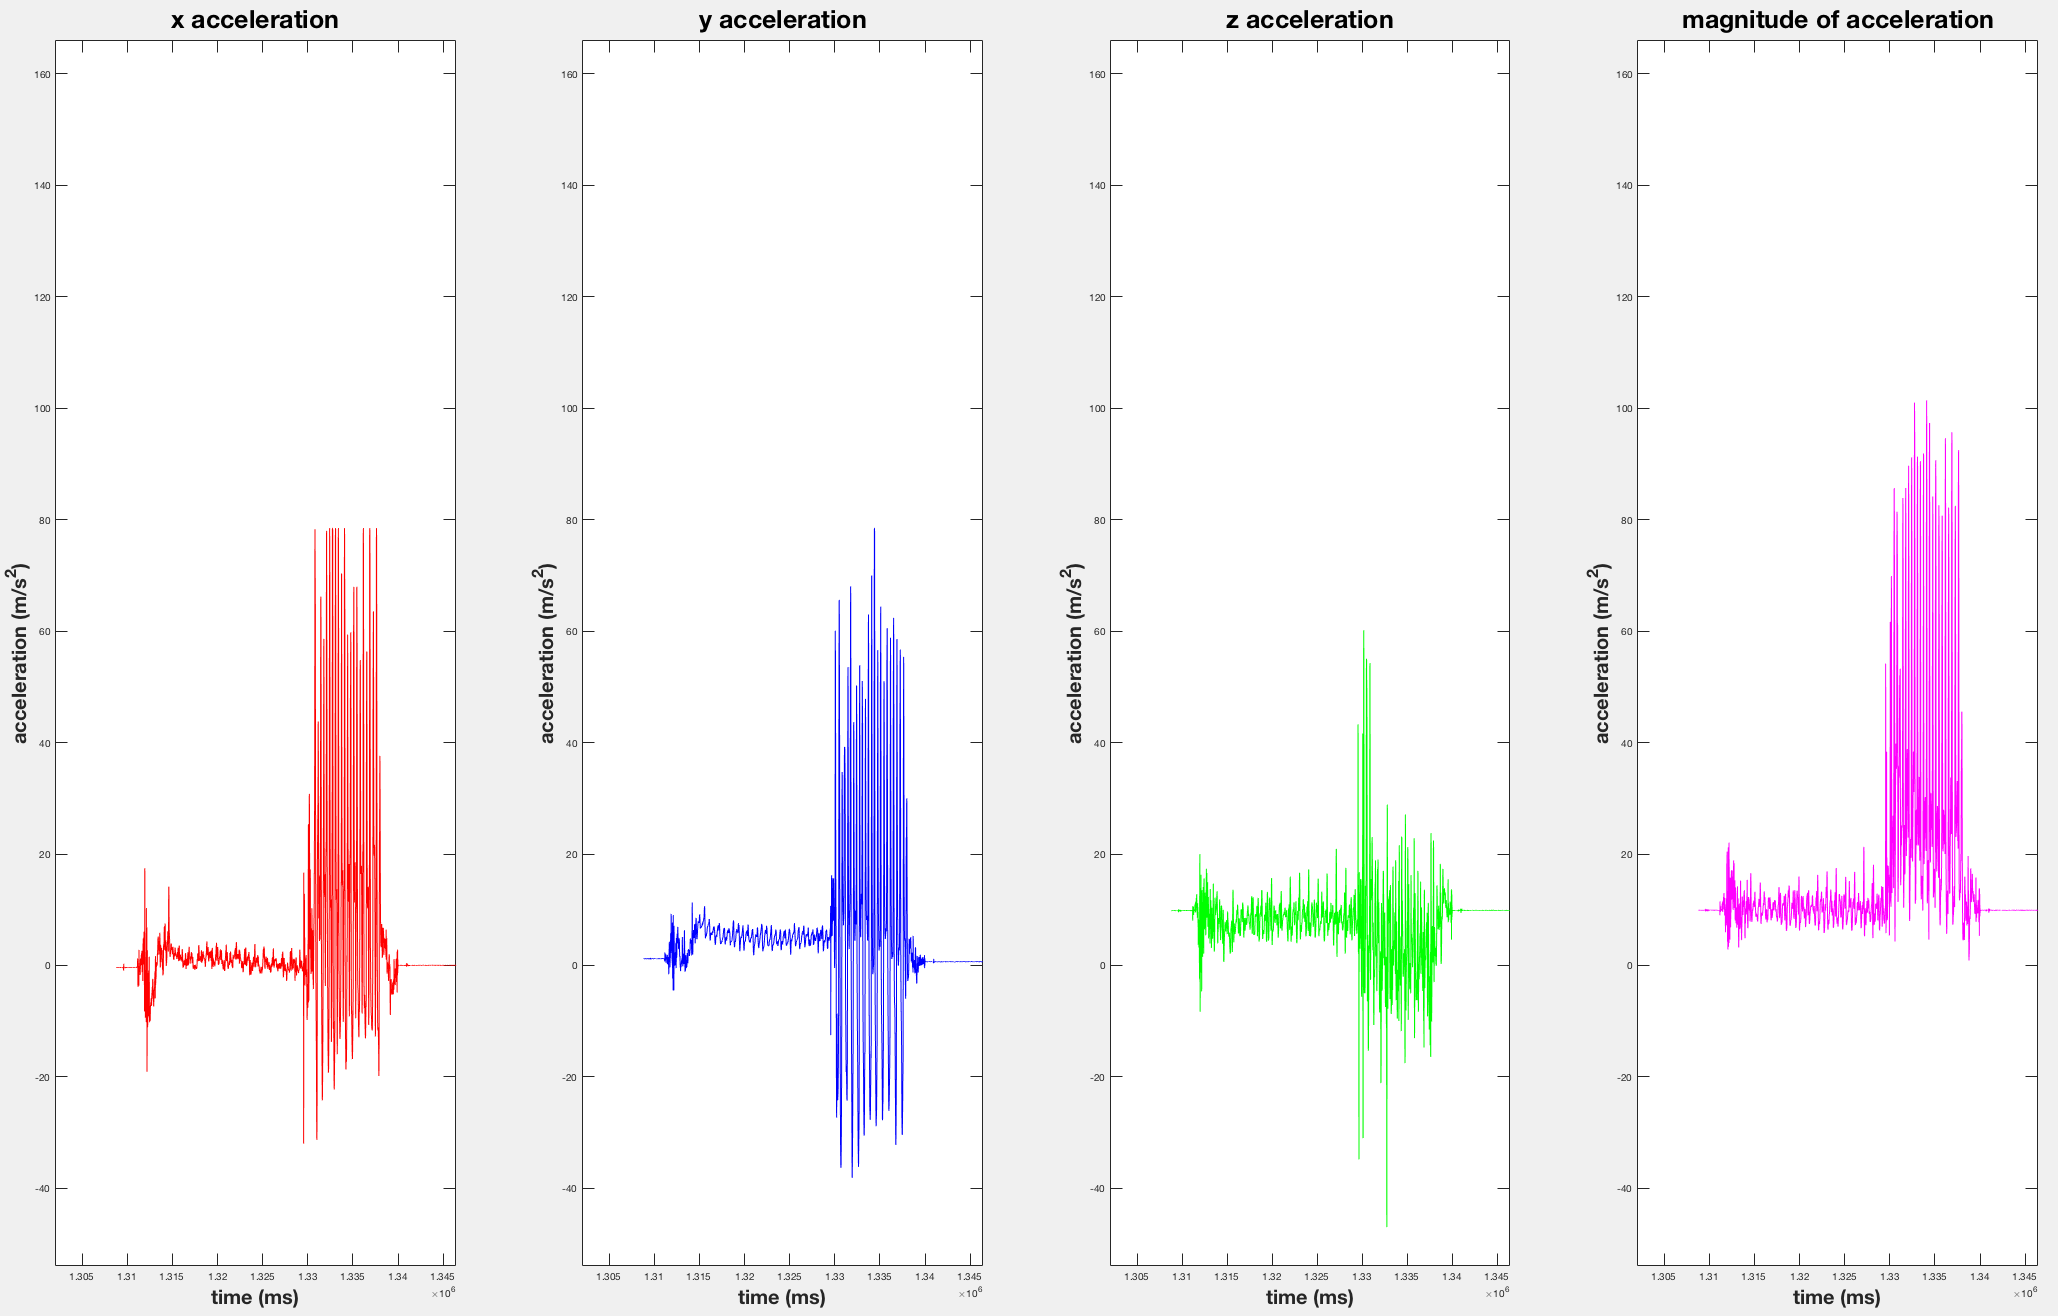
\includegraphics[width=1.0\columnwidth]{pos_acc_separated.png}
\caption{The above plots are x, y, z and magnitude of acceleration, respectively, of one theft instance.}
\end{figure}

\begin{figure}[H]
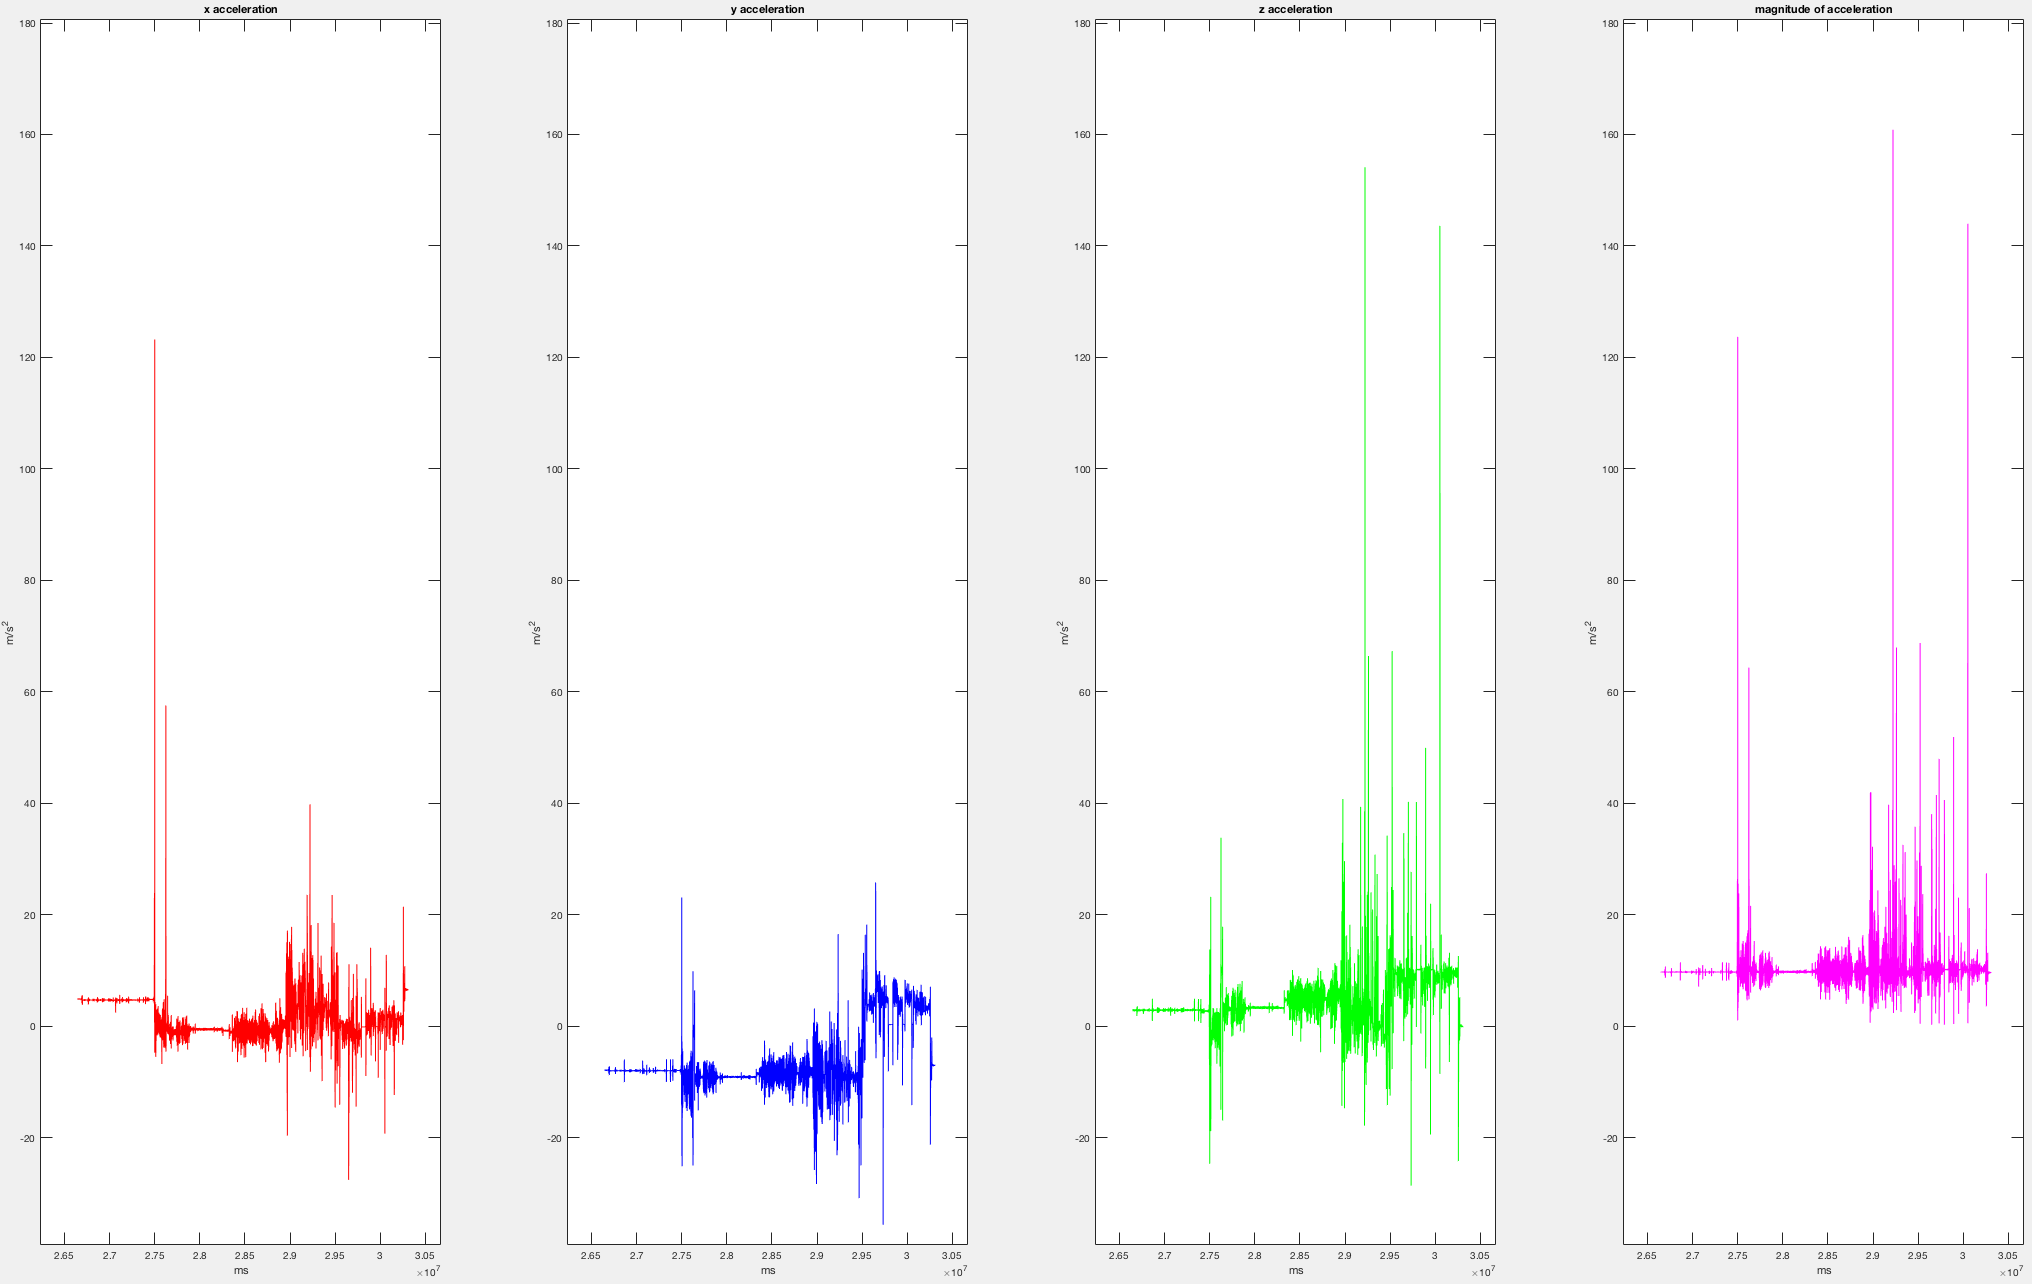
\includegraphics[width=1.0\columnwidth]{neg_acc_separated.png}
\caption{The above plots are x, y, z and magnitude of acceleration, respectively, during normal usage at an arbitrary time period.}
\end{figure}



\subsection{Machine Learning Algorithms}
We evaluate three standard machine learning algorithms: linear SVM, logistic regression and random forest, provide by the Python scikit-learn library, on their efficacy of distinguishing between theft and normal usage. 
In order to mitigate the fact that we have many more negative samples than positive ones, we tweak the class weight, a class attribute built in the scikit-learn library, to produce different ratios of negative and positive class weights used in training, for example 1 : 1, 1 : 8000, and `balanced,' which adjusts the class weights to be inversely proportional to class frequencies in the input data.



\section{Results}
We ran a 10-fold cross validation on the entire dataset describled in the Feature Selection section, which consists of 60 positive samples and approximately 248,000 negative samples. 
Among the three classifiers, logistic regression performs the best in terms of producing the lowest false negative rate and the highest true positive rate. 
Besides class weights, another parameter we finetune in training is the window size \textit{n}. 
Confusion matrices of logistic regression with class weight = {0: 1.0, 1: 200.0}, random forest with class weight = {0: 1.0, 1: 5000.0} and linear SVM with class weight = {0: 1.0, 1: 1000.0} when the window size \textit{n} = 2 second are shown below.

\begin{table}[H]
\centering
\begin{tabular}{@{}lll@{}}
\toprule
              & Predicted Negative & Predicted Positive \\ \midrule
True Negative & 248223             & 170                \\
True Positive & 0                  & 60                 \\ \bottomrule
\end{tabular}
\caption{Confusion Matrix of Logistic Regression}
\label{my-label}
\end{table}

\begin{table}[H]
\centering
\begin{tabular}{@{}lll@{}}
\toprule
              & Predicted Negative & Predicted Positive \\ \midrule
True Negative & 248360             & 33                 \\
True Positive & 32                 & 28                 \\ \bottomrule
\end{tabular}
\caption{Confusion Matrix of Random Forest}
\label{my-label}
\end{table}

\begin{table}[H]
\centering
\begin{tabular}{@{}lll@{}}
\toprule
              & Predicted Negative & Predicted Positive \\ \midrule
True Negative & 246522             & 1871               \\
True Positive & 42                 & 18                 \\ \bottomrule
\end{tabular}
\caption{Confusion Matrix of Linear SVM}
\label{my-label}
\end{table}


The logistic regression classifier has a false negative rate of 0.6844\%, which means that on average users receive 1 false alarm every week, and a true positive rate of 100\%. For our purpose of smartphone theft detection, linear SVM's false negative rate is too hight.

We also compute feature rankings to find the most predictive features for each classifier. 
For logistic regression, to calculate feature scores that are invariant to scaling feature values, we adjust the coefficient of each feature in the decision function by multipling it by the standard deviation of the values of this feature across all instances in the training set. 
Then we get the adjusted coefficients as the feature importances of logistic regression as -2.73319487, 0.0129842047, 0.477534932, -0.0143829911, -1.18427357, -0.0470492037, 0.0580951517, 0.880738694, 0.666823228, \\-0.937781183, 0.273227115, -2.69540663, from which we can tell the most representative features are maximum, and arc length in the before-window and product of arc length and standard deviation in the after-window. 
For random forest, we use the built-in attribute feature importances in the scikit-learn library, which estimate the relative importance of the features by computing the expected fraction of the samples they contribute to. 
Thus the higher in the tree, the more important the feature is \cite{sklearn:rfdoc}. 
We get the feature importances of random forest as 0.04751106, 0.0080411, 0.02881483, 0.01533719, 0.02245781, 0.03309431, 0.12388036, 0.20288397, 0.16426152, 0.21908845, 0.05162059, 0.0830088.

Another way to visulize the representative features is to plot a histogram of dataset and to see which features can better seperate the positive and negative data points, as shown in Figures 1 and 2.

\begin{figure}[H]
\begin{center}
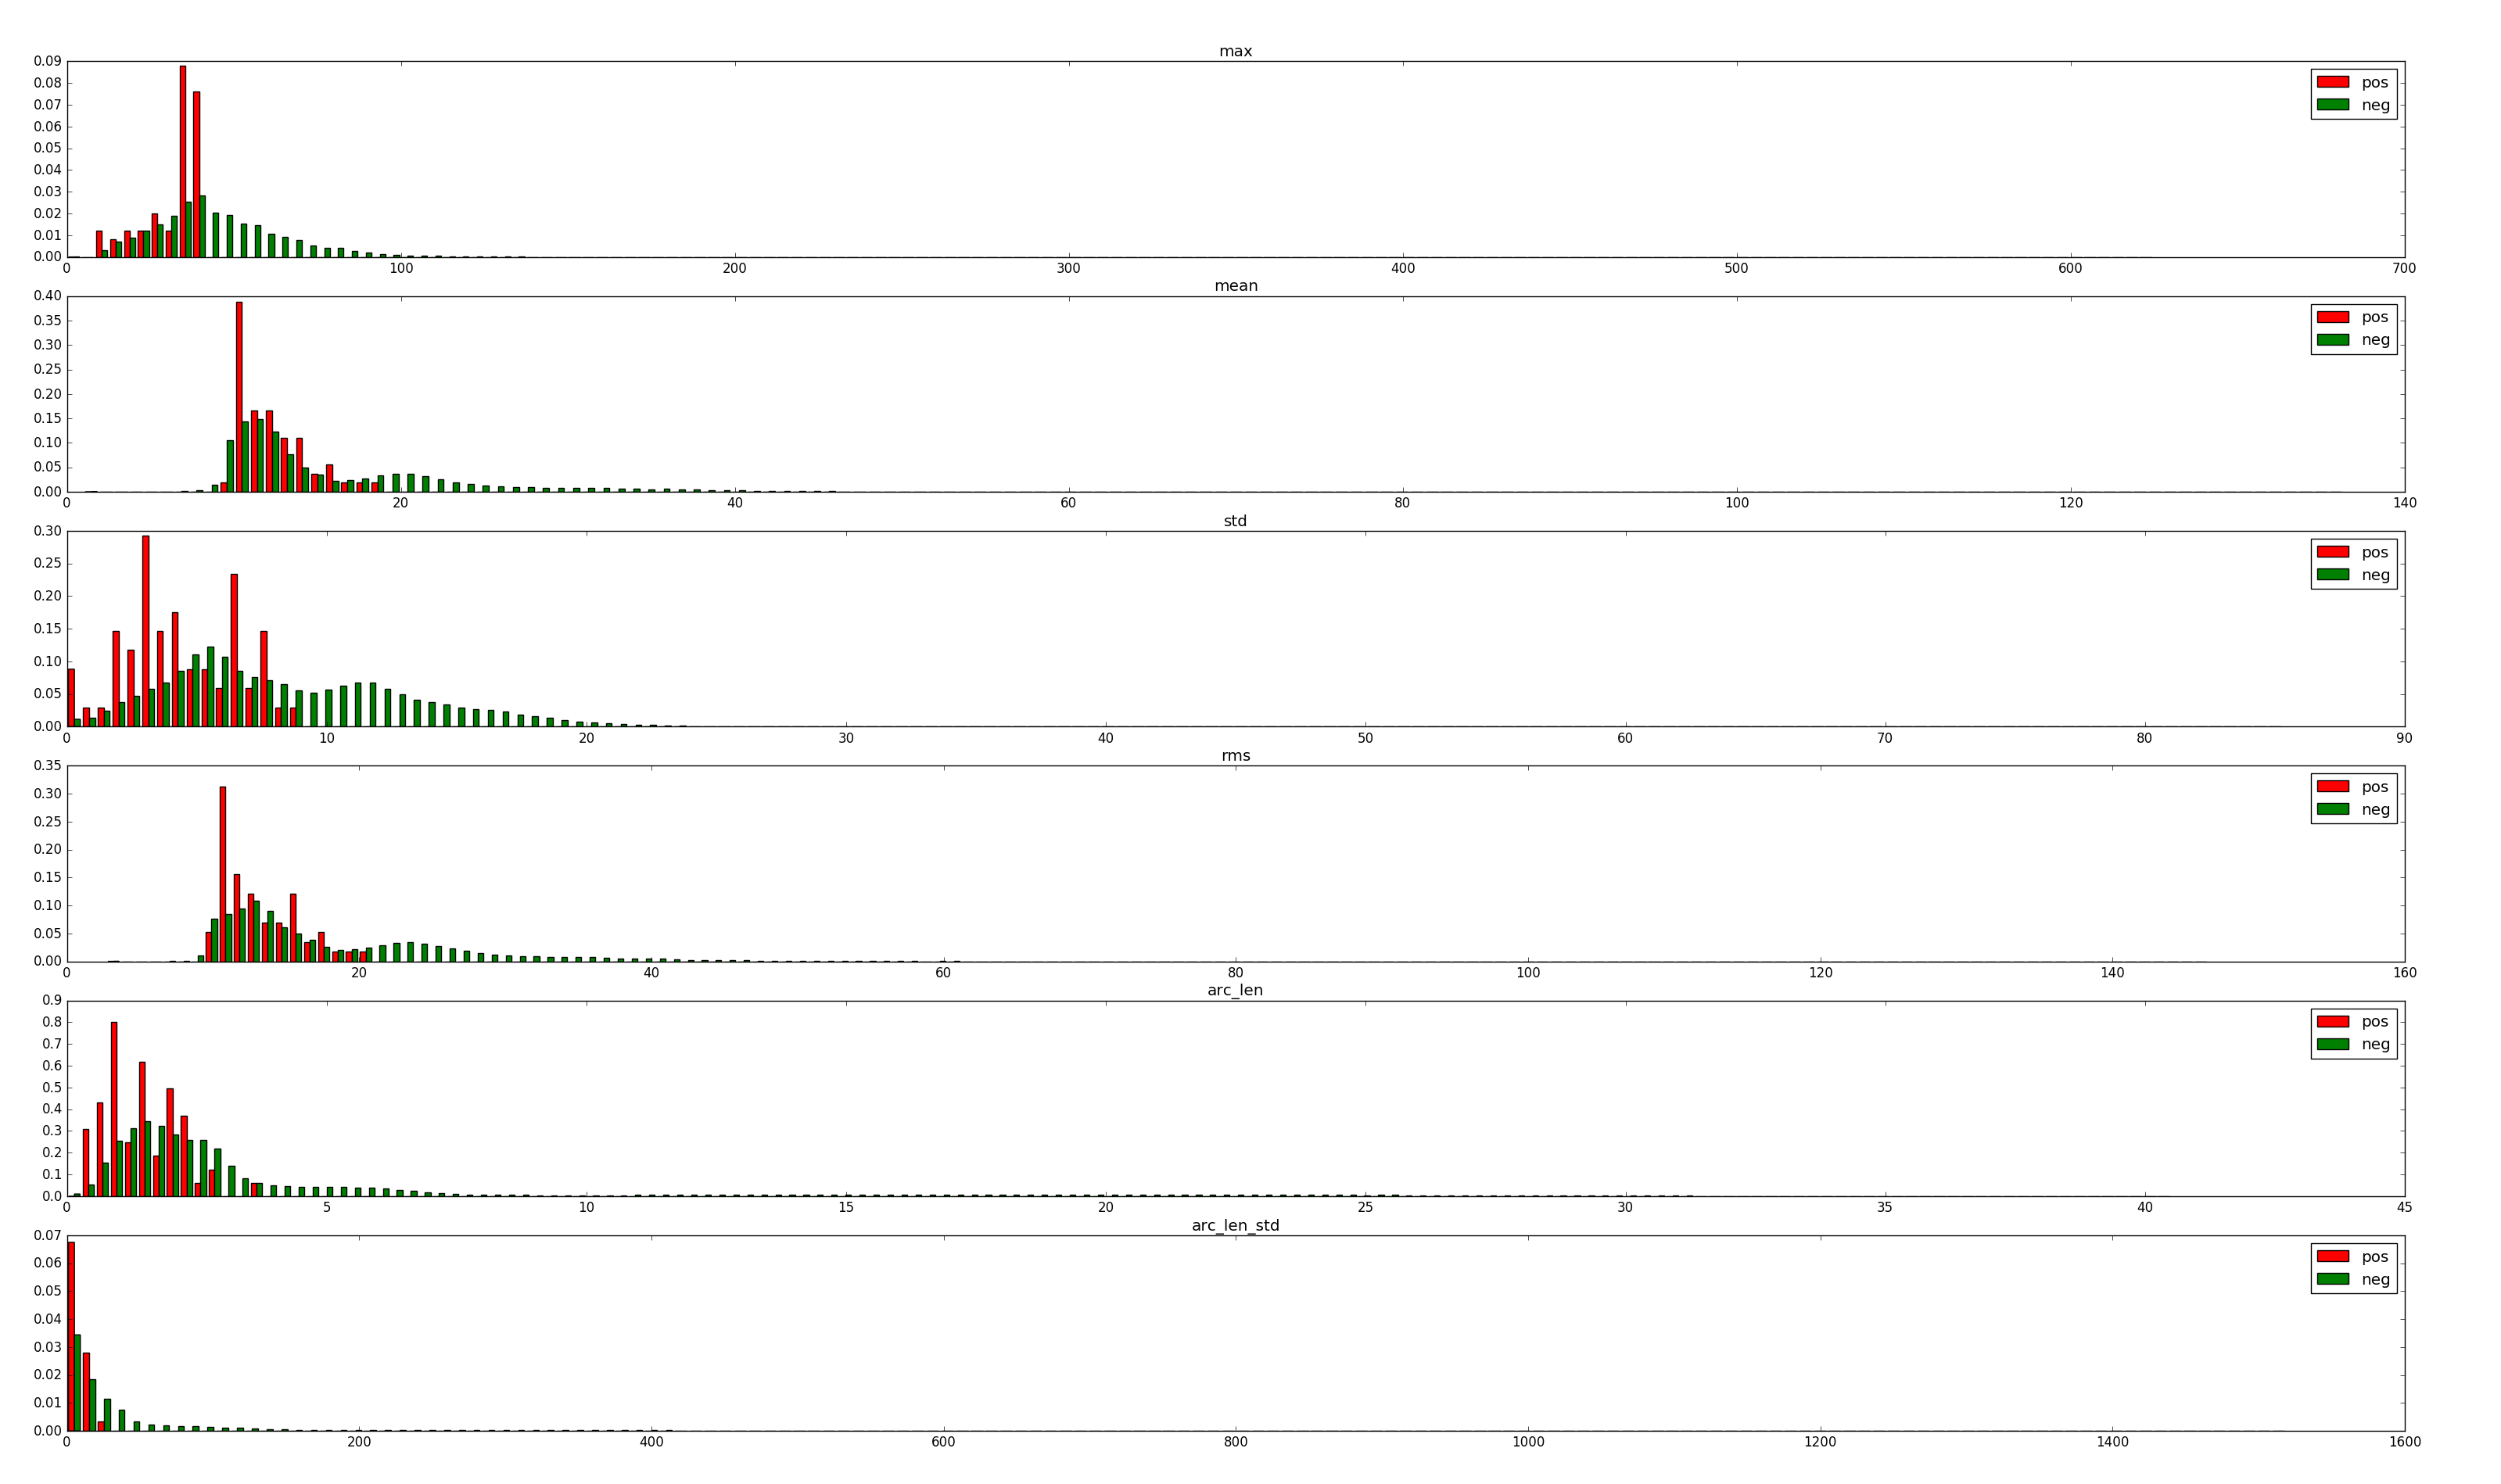
\includegraphics[width=1.0\columnwidth]{hist_features_before_win_size_1_2.png}
\end{center}
\caption{histogram of features in 1-second windows before \textit{40 $m/s^2$} thresholds.}
\end{figure}

\begin{figure}[H]
\begin{center}
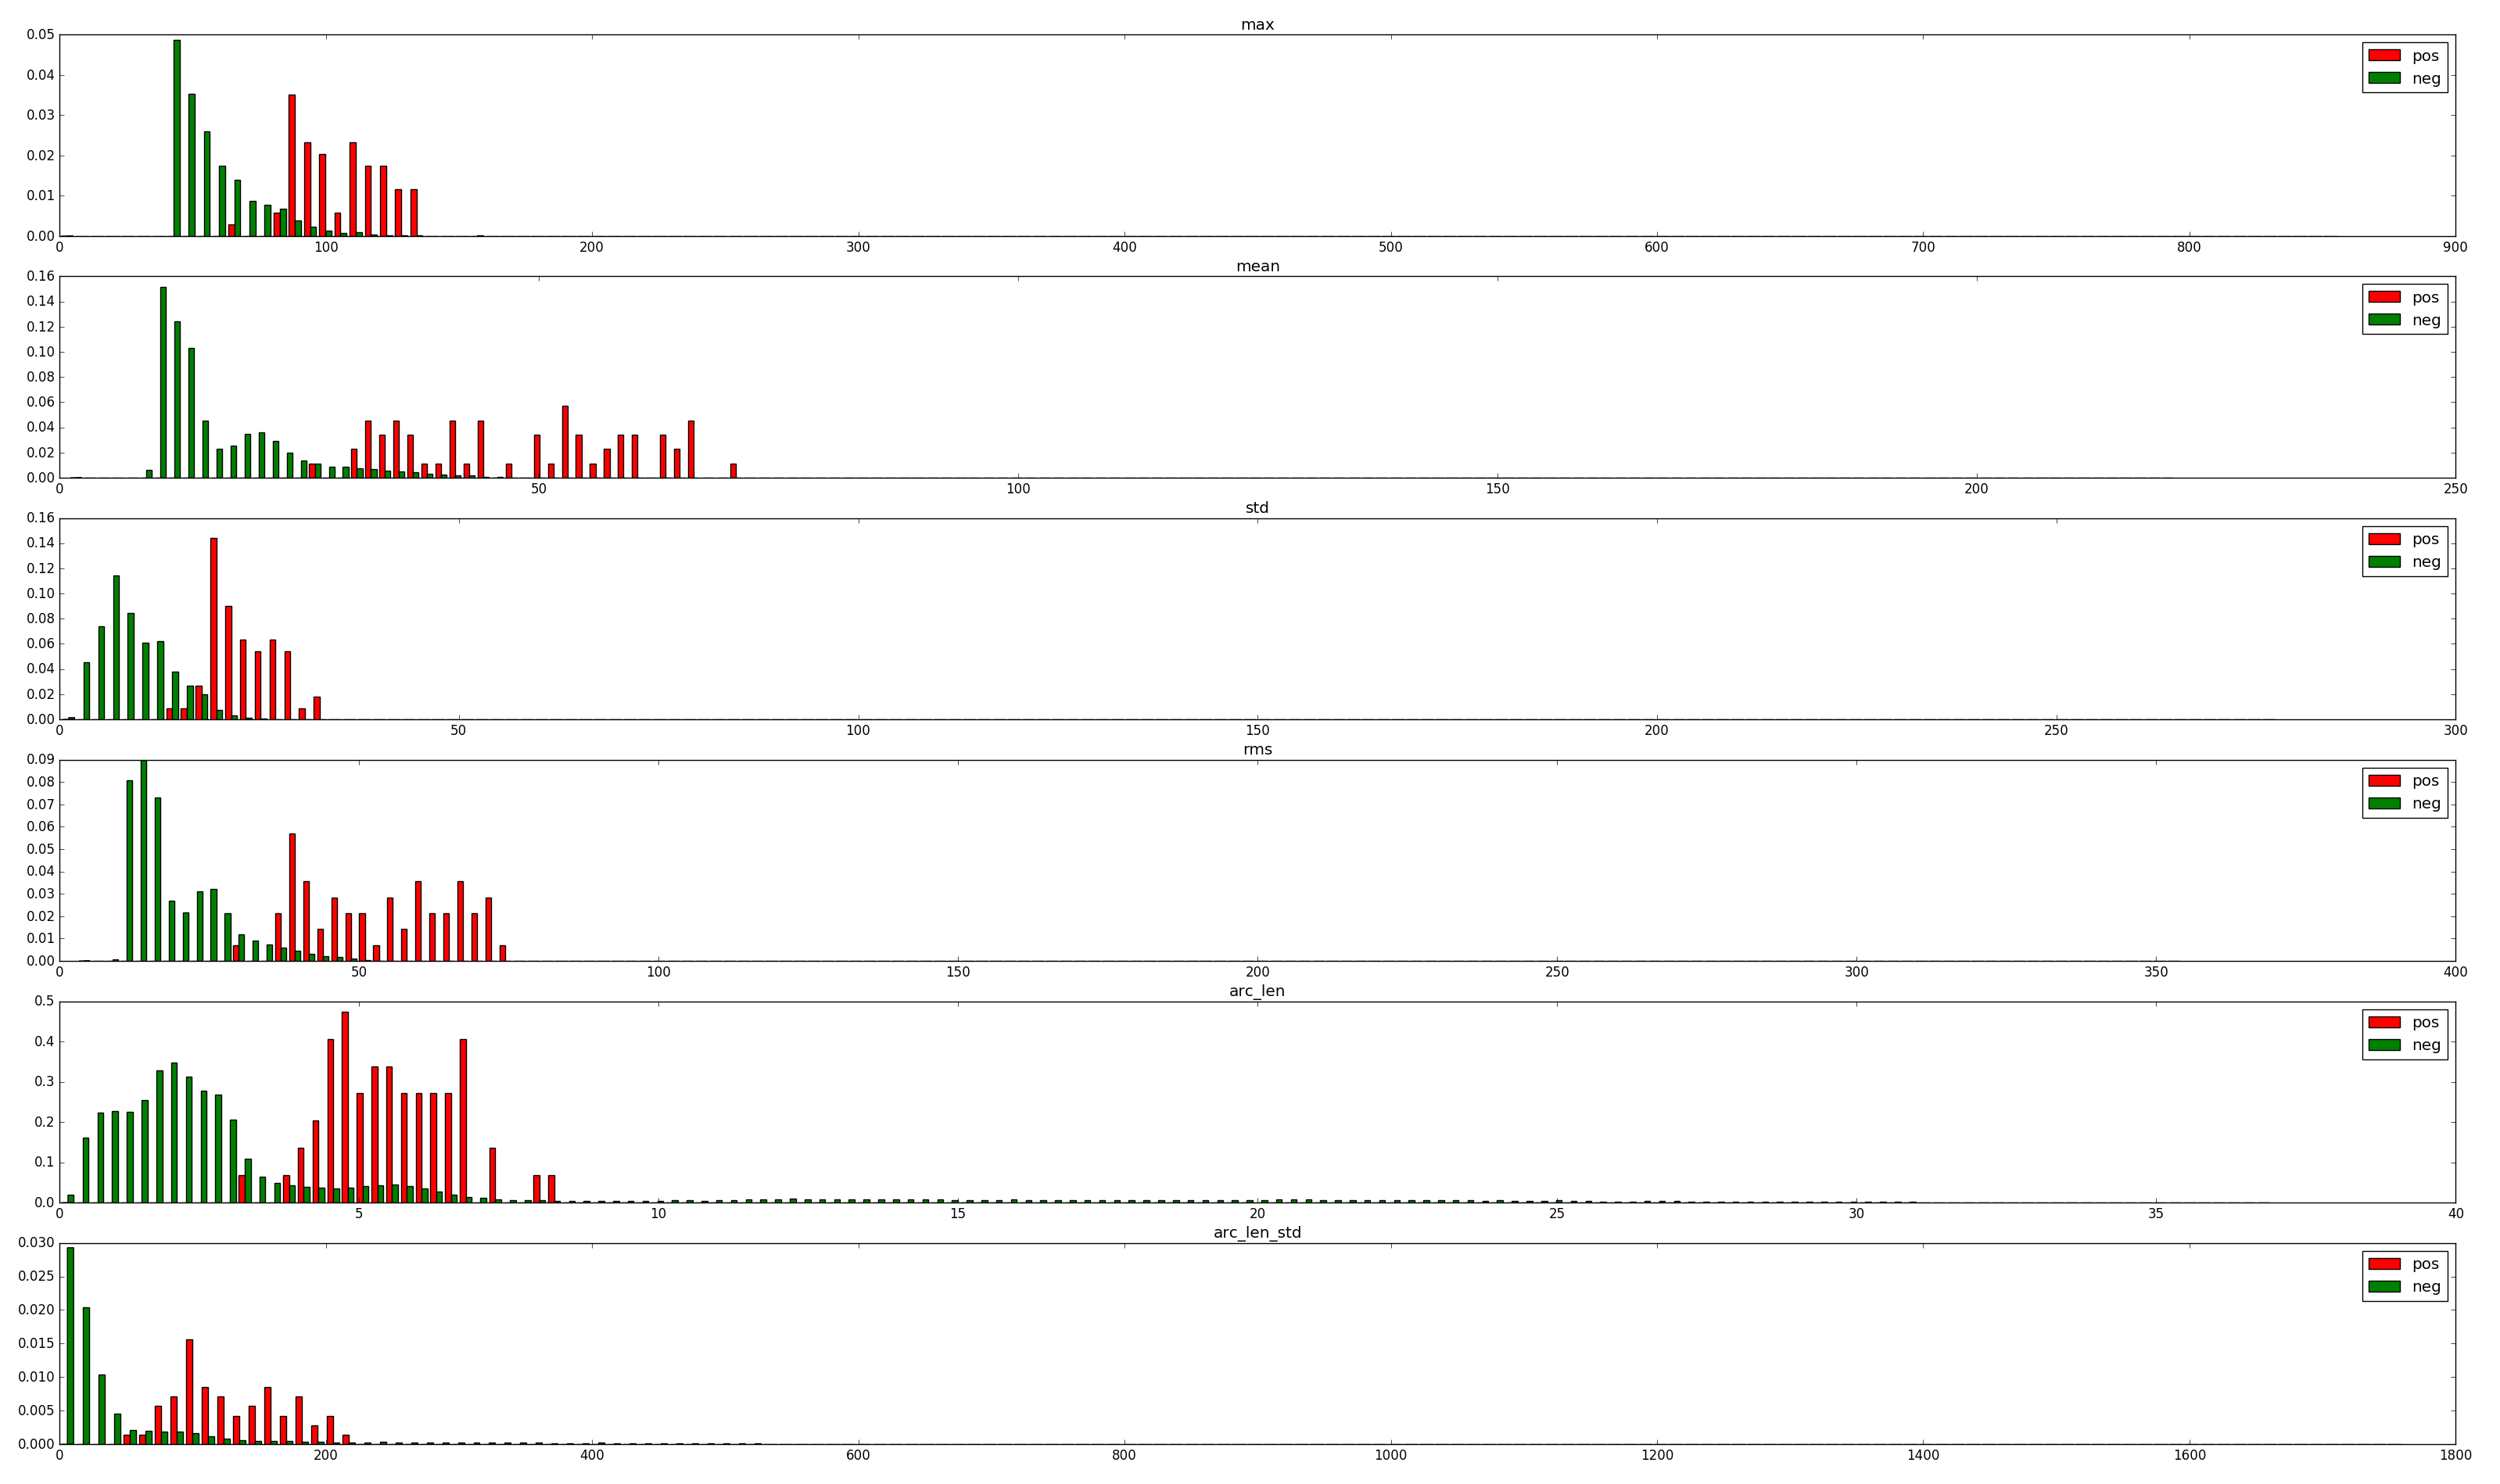
\includegraphics[width=1.0\columnwidth]{hist_features_after_win_size_1_2.png}
\end{center}
\caption{histogram of features in 2-second windows after \textit{40 $m/s^2$} thresholds.}
\end{figure}

To compare the performance of random forest and logistic regression, we finetune the class weight of logistic regrssion classifier to lower its true positive rate until it is approximately the same as random forest classifier, then we compare the number of false postive instances of the two classiifier. 
As a result, at a 41.7\% true positive rate (25 true positive instances), logistic regression with class weigth = {0: 1.0, 1: 2.0} has 34 false positive instances. 
At a 46.7\% true positive rate (28 true positive instances), random forest with class weight = {0: 1.0, 1: 5000.0} has 33 false positive instances. 
Thus the performance of logistic regression is at least as good as random forest.
We also include the Receiver Operating Characteristic (ROC) curves of the two classifiers. \textcolor{red}{ add ROC of random forest and logistic regression }




\section{Discussion}
In this work, we demonstrate that with proper feature extraction we can use accelerometer data alone to detect common smartphone theft, such as pickpocket and grab-and-run, without sacrificing user experience. 
In the future, in addition to accelerometer, we propose to utilize other intrinsic-sensor available on a smartphone, such as step count and try using techiques, such as time interpolation and filtering to preprocess raw sensor data for better performance. 
We would also like to collect more positive samples to have a more diverse theft dataset that covers more theft scenarios and test our models on a hold-out test set. 
We are interested in deploying theft detector on a smartphone and test it real time performance.




\section{Acknowledgments}
\textcolor{red}{Comment out for double blind review}. 

The authors would like to thank Prakash P. Bhasker and Micah J. Sheller for proivding with the Android sensor monitoring software, Jennider Chen from the Good Research for her assistance on conducting the user study, and Irwin Reyes \textcolor{red}{Who else gives feedback to draft} for giving feedback. 
This research was conducted at The Intel Science and Technology Center for Secure Computing (http://scrub.cs.berkeley.edu/) at UC Berkeley. 
The work is supported by \textcolor{red}{What Grants and Funds}. 




% The following two commands are all you need in the
% initial runs of your .tex file to
% produce the bibliography for the citations in your paper.
\bibliographystyle{abbrv}
\bibliography{sigproc}  % sigproc.bib is the name of the Bibliography in this case
% You must have a proper ".bib" file
%  and remember to run:
% latex bibtex latex latex
% to resolve all references
%
% ACM needs 'a single self-contained file'!

\end{document}
